\section{Brownian Motion}

\begin{frame}{Brownian motion}
Brownian motion can be constructed as a limit of random walks.
\begin{eqnarray*}
 P(Y_i=\Delta x)=\frac{1}{2} \\
 P(Y_i=-\Delta x)=\frac{1}{2}
\end{eqnarray*}
\pause

\begin{center}
What is the distribution of 
\begin{equation*}
X_n=Y_1+Y_2+...+Y_n
\end{equation*}
if $Y_1,Y_2,...,Y_n$ are i.i.d.? 
\end{center}
\end{frame}


\begin{frame}
\begin{eqnarray*}
X_n&= &Y_1+Y_2+...+Y_n\\ \\
\pause
\ln (M_{X_n})(\lambda)&\approx &\frac{(\Delta x)^2}{\Delta t} \left(\frac{\lambda ^2 T}{2}+\frac{\lambda ^4 \Delta x ^2 T}{4}+... \right)\\
\end{eqnarray*}
\pause
If we assume that $\frac{(\Delta x)^2}{\Delta t}=k$ then,
\begin{equation*}
\lim_{\Delta x \to 0}{M_{X_n}(\lambda)}=\exp\left(\frac{kT\lambda ^2}{2}\right)
\end{equation*}
which means $X_n \sim N(0,kT)$
\end{frame}

\begin{frame}
\begin{block}{Standard Brownian Motion}
A random variable $B(t)$ that depends continuously on $t \in [0,T]$ and satisfies: 
\begin{itemize}
\item $B(0)=0$
\item For $0 \leq s<t\leq T$: $B(t)-B(s)\sim N(0, t-s)$
\item For $0 \leq s<t<u<v\leq T$ the increments $B(t)-B(s)$ and $B(v)-B(u)$ are independent.
\end{itemize}
\end{block}
\end{frame}

\begin{frame}{Computational Purposes}
Discretized Brownian motion: $B(t)$ is specified at discrete t values.
\begin{eqnarray*}
&& W(0)=0\\
&& W(j)=W(j-1)+dW(j)
\end{eqnarray*}
$dW(j)$ is an independent random variable of the form $N(0,\Delta t)$
\end{frame}

\begin{frame}
\begin{center}
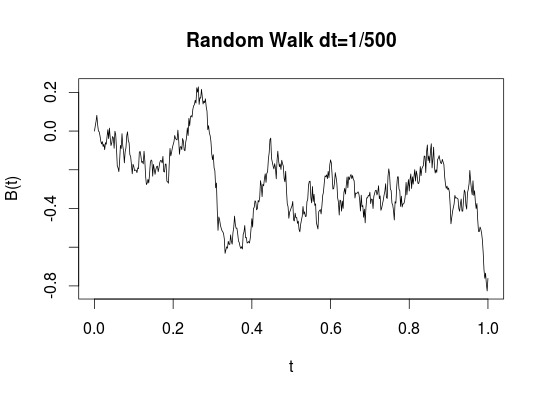
\includegraphics[scale=0.5]{r_w_3.png}
\end{center}
\end{frame}

\begin{frame}
\begin{center}
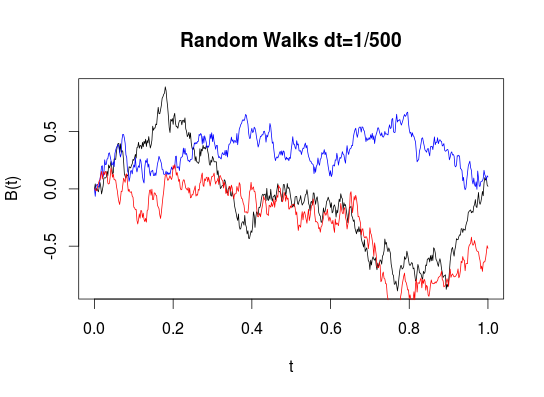
\includegraphics[scale=0.5]{r_w_4.png}
\end{center}
\end{frame}

\begin{frame}
\begin{center}
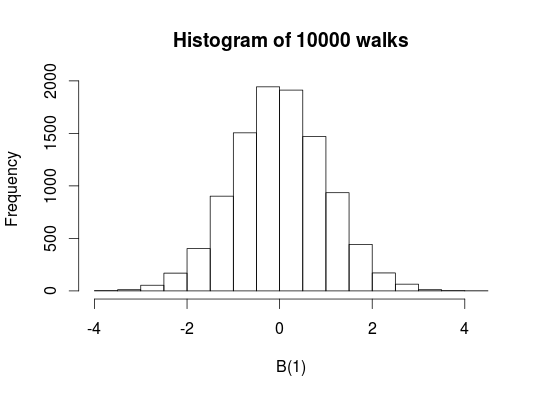
\includegraphics[scale=0.5]{hist.png}
\end{center}
\end{frame}

\begin{frame}
\begin{center}
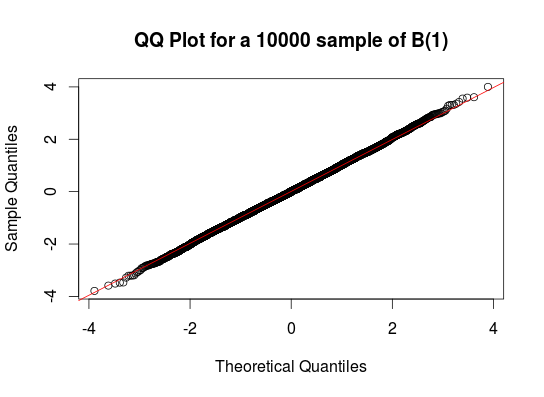
\includegraphics[scale=0.5]{qqplot.png}
\end{center}
\end{frame}


\section{Stochastic Integrals}

\begin{frame}{Stochastic Integrals}
\pause
\begin{center}
What does $\int_{a}^{b} f(t)dB$ mean? \bigskip \pause  $\int_{a}^{b} B(t)dB$?\pause \\

¿An analogy of the Riemann-Stietjes sum?\\ \pause 
%\begin{equation*}
%\sum_{i=1}^{n}B(t_{j-1})\left( B(t_{j})-B(t_{j-1})\right) 
%\end{equation*}
%\pause
\bigskip

In $[0,T]$ with $\Delta t=1/500$:\\ \pause
$It\hat{o}=-0.42765$\\ \pause
$Stratonovich=0.088892$
\end{center}
\end{frame}

%\begin{frame}
%Consider the following functions:
%\[1_{[t_{i-1},t_i)} = \left \{
%  \begin{array}{lr}
%1, & t \in [t_{i-1},t_i)\\
%0, & otherwise
%  \end{array}
%\right.
%\]

%$$f_n=\sum_{i=1}^{n}a_i1_{[t_{i-1},t_i)} $$\\

%We define the stochastic integral as:
%$$I(f_n):=\sum_{i=1}^{n} a_i(B(t_i)-B(t_{i-1}))$$
%\end{frame}

\begin{frame}
\begin{block}{Definition}
Given f(t) a continuous function with bounded variation. Let $a_i=f(t_{i-1})$, then \textbf{the Weiner integral} is:
\begin{equation*}
I(f):=\lim_{n \to \infty}\sum_{i=1}^{n}a_i(B(t_i)-B(t_{i-1}))
\end{equation*}
\pause
\begin{itemize}
\item $E[I(f)]=0$
\item $Var[I(f)]=\int_{a}^{b}f^2(t)dt$
\end{itemize}
\end{block}

%\begin{eqnarray*}
%E[I(f)]&=&0\\
%Var[I(f)]&=&\int_{a}^{b}f^2(t)dt
%\end{eqnarray*}
\end{frame}
